\documentclass[11pt,oneside,a4paper]{article}
\usepackage[utf8]{inputenc}
\date{}
\usepackage[linesnumbered,ruled,vlined]{algorithm2e}
\SetKwInput{KwInput}{Input}                % Set the Input
\SetKwInput{KwOutput}{Output}              % set the Output<z
\usepackage{blindtext}
\usepackage{changepage}


\usepackage[formats]{listings}  %% Code listing%% Code format

%\usemintedstyle{friendly}
\usepackage{amsmath}
\usepackage{color}
\usepackage{tcolorbox}
\usepackage{sectsty}
\usepackage{stmaryrd}
\usepackage{gensymb}
\usepackage{wasysym}
\usepackage{amsfonts}
\usepackage{xcolor}
\usepackage{tikz}
\usetikzlibrary{shapes,snakes}
\usepackage{graphicx}
\usepackage{stmaryrd}
\usepackage{mathtools}
\usepackage{amsthm}
\usepackage{caption}
\usepackage{subcaption}
\usepackage[margin=1.2in]{geometry}
%__________WIDE HAT_________
\usepackage{scalerel,stackengine}
\stackMath
\newcommand\reallywidehat[1]{%
\savestack{\tmpbox}{\stretchto{%
  \scaleto{%
    \scalerel*[\widthof{\ensuremath{#1}}]{\kern-.6pt\bigwedge\kern-.6pt}%
    {\rule[-\textheight/2]{1ex}{\textheight}}%WIDTH-LIMITED BIG WEDGE
  }{\textheight}%
}{0.5ex}}%
\stackon[1pt]{#1}{\tmpbox}%
}
\parskip 1ex
%______________________________
\usepackage{hyperref}
\hypersetup{
    colorlinks=true,
    urlcolor=blue
}
\setlength{\parindent}{0in}
\theoremstyle{definition}
\newtheorem{definition}{Definition}[section]

\theoremstyle{remark}
\newtheorem*{remark}{Remark}
\usepackage{amsmath}
\usepackage[T1]{fontenc}
\usepackage{float}
\usepackage[british,UKenglish,swedish,USenglish,english,american]{babel}
\usepackage[T1]{fontenc}
\usepackage{fancyhdr}
\usepackage{natbib}
%\pagestyle{fancy}
\begin{document}
\renewcommand{\bibname}{References}
\hypersetup{citecolor=black}
\begin{titlepage}\centering
\vspace*{\fill}
\Huge Assignment 3\\
\vspace*{10mm}
\large Includes methods of Directed Graphical Models, Expectation Maximisation, Dynamic programming, Variational Inference, Hidden Markov Models and Spectral Graph Analysis\\
\vspace*{\fill}
\large \textsc{DD2434 Advanced Machine Learning} \\
\textsc{Filip Bergentoft, bergento@kth.se} \\
\end{titlepage}

\newpage
\section*{3.1 Easier EM for Advertisements}
Submitted a solution to the original version of 3.1 before it was simplified and received full points plus $\frac{1}{4}$ bonus points for my solution.

\section*{3.2 Hard EM for Advertisements}
Problem removed from assignment.
qqq: Add how I have chosen to do at the root/leaves when it comes to the Normal Dist
\section*{3.3 Complicated likelihood for leaky units on a tree}
\begin{tcolorbox}
  \textbf{Problem formulation:} Consider the following model. A binary tree $T$ has random variables associated with its vertices. A vertex $u$ has an observable variable $X_{u}$ and a latent class variable $Z_{u} .$ Each class $c \in[C]$ has a normal distribution $N\left(\mu_{k}, \sigma^{2}\right) .$ If the three neighbors of $u$ are $v_{1}, v_{2},$ and $v_{3},$ then
  $$
  p\left(X_{u} \mid Z_{u}=c, Z_{v_{1}}=c_{1}, Z_{v_{2}}=c_{2}, Z_{v_{2}}=c_{2}\right) \sim N\left(X_{u} \mid(1-\alpha) \mu_{c}+\sum_{i \in[3]} \frac{1}{3} \alpha \mu_{c_{i}}, \sigma^{2}\right)
  $$
  The class variables are iid, each follows the categorical distribution $\pi .$ Provide a linear time algorithm that computes $P(X \mid T, M, \sigma, \alpha, \pi)$ when given a tree $T$ (with vertices $V(T))$, observable variables for its vertices $X=\left\{X_{v}: v \in V(T)\right\},$ and parameters $M=\left\{\mu_{c}: c \in[C]\right\}, \sigma, \alpha .$
\end{tcolorbox}
We are interested in finding the likelihood of our observations $X$ by marginalising the following
\begin{equation}
  p(X) = \sum_Z p(X,Z)
\end{equation}
where $\sum_Z$ denotes the sum over all latent variables. We will show how this problem can be continuously split up into smaller and smaller subproblems using the structure of the binary tree until the leaves are reached. This will result in a linear algorithm for computing the requested likelihood $P(X \mid T, M, \sigma, \alpha, \pi)$ which we will from now on denote as $p(X)$ for the sake of brevity.

\subsection*{Starting at the root}
We will start by showing how one can split the problem into two subproblems when starting at the root.

Let $u$ denote the root and $u_1, u_2$ denote its children as in figure \ref{root_case}.
\begin{figure}[H]
\begin{center}
  \scalebox{0.7}{
  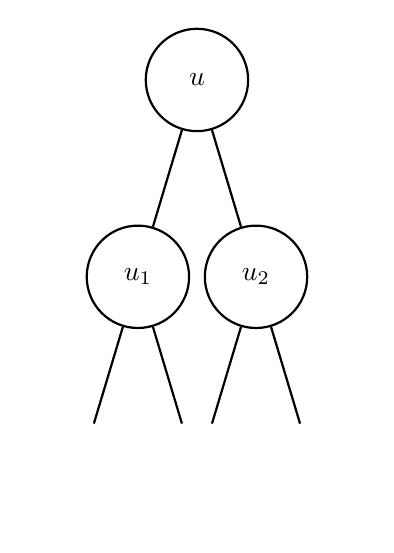
\begin{tikzpicture}[thick, minimum size=1.3cm, level distance=2.5cm]
    \node[circle,draw]{$u$}
        child { node[circle,draw]{$u_1$}
            child { node[circle]{}}
            child { node[circle]{}}
        }
        child { node[circle,draw]{$u_2$}
            child { node[circle]{}}
            child { node[circle]{}}
        };
  \end{tikzpicture}
  }
\end{center}
\caption{Binary tree starting at root r, branches below $u_1, u_2$ denotes subtrees}
\label{root_case}
\end{figure}

We begin by using that the root $u$ is independent of its children given $Z_u, Z_{u_1}, Z_{u_2}$ which leads to the following factorisation.
\begin{align}
  p(X) & = \sum_Z p(X,Z) = \sum_Z p(X_u, X_{u_1}, X_{u_2}, X_{u_1\downarrow}, X_{u_2\downarrow}, Z) \nonumber \\
  & = \sum_Z p(X_u, X_{u_1}, X_{u_2}, X_{u_1\downarrow}, X_{u_2\downarrow}, Z_{u_1\downarrow}, Z_{u_2\downarrow}| Z_u, Z_{u_1}, Z_{u_2})p(Z_u, Z_{u_1}, Z_{u_2}) \nonumber\\
  & = \sum_Z p(X_u|Z_{u_1}, Z_{u_2}, Z_u) p(Z_{u_1}, Z_{u_2}, Z_u)
  p(X_{u_1}, X_{u_1 \downarrow}, Z_{u_1 \downarrow}|Z_{u_1}, Z_u)
  p(X_{u_2}, X_{u_2 \downarrow}, Z_{u_2 \downarrow}|Z_{u_2}, Z_u) \nonumber\\
\end{align}
We can now let the sums over $Z_{u_1 \downarrow}$ and $Z_{u_2 \downarrow}$ move in which yields that
\begin{align}
  p(X) & = \sum_{Z_u, Z_{u_1}, Z_{u_2}}\bigg[p(X_u|Z_{u_1}, Z_{u_2}, Z_u) p(Z_{u_1}, Z_{u_2}, Z_u) \nonumber\\
  & \qquad\qquad\quad \Big(\sum_{Z_{u_1 \downarrow}} p(X_{u_1}, X_{u_1 \downarrow}, Z_{u_1 \downarrow}|Z_{u_1}, Z_u) \Big)\Big(\sum_{Z_{u_2 \downarrow}} p(X_{u_2}, X_{u_2 \downarrow}, Z_{u_2 \downarrow}|Z_{u_2}, Z_u) \Big)\bigg] \nonumber \\
\end{align}
Using that the latent variables $Z$ are independent given $\pi$ and substituting for the available densities yields
\begin{align}
  p(X) & = \sum_{Z_u, Z_{u_1}, Z_{u_2}}\bigg[\mathcal{N}\Big(X_u|(1-\alpha)\mu_{Z_u} +\frac{\alpha}{2}(\mu_{Z_{u_1}}+\mu_{Z_{u_2}}), \sigma^2 \Big) \pi(Z_u) \pi(Z_{u_1}) \pi(Z_{u_2})\\
  & \qquad\quad
  \Big(\underbrace{\sum_{Z_{u_1 \downarrow}} p(X_{u_1}, X_{u_1 \downarrow}, Z_{u_1 \downarrow}|Z_{u_1}, Z_u)}_\text{$p_{Z_{u_1 \downarrow}}$} \Big)
  \Big(\underbrace{\sum_{Z_{u_2 \downarrow}} p(X_{u_2}, X_{u_2 \downarrow}, Z_{u_2 \downarrow}|Z_{u_2}, Z_u)}_\text{$p_{Z_{u_2 \downarrow}}$} \Big) \bigg]
\end{align}
Where $p_{Z_{u_1 \downarrow}}$ and $p_{Z_{u_2 \downarrow}}$ denotes two independent subproblems with respect to the sets of latent variables $Z_{u_1 \downarrow}$ and $Z_{u_2 \downarrow}$

\subsection*{Starting at a node within the tree}
Now we will show how we can continue to divide each subproblem $p_{Z_{u_1 \downarrow}}$ and $p_{Z_{u_2 \downarrow}}$ defined above until the leaves are reached. We will now let $u_{1}$ and $u_{2}$ be the children of node $u$ and we will treat the problem shown in figure \ref{within_tree}


\begin{figure}[H]
\begin{center}
  \scalebox{0.7}{
  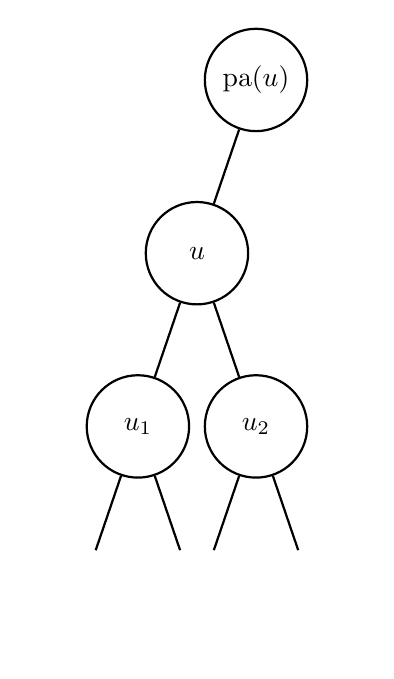
\begin{tikzpicture}[thick, minimum size=1.3cm, level distance=2.2cm]
    \node[circle,draw]{pa$(u)$}
        child { node[circle,draw]{$u$}
            child { node[circle,draw]{$u_1$}
                child { node[circle]{} }
                child { node[circle]{} }
                }
            child { node[circle,draw]{$u_2$}
                child { node[circle]{} }
                child { node[circle]{} }
                }
        }
        child [ missing ];
  \end{tikzpicture}
  }
\end{center}
  \caption{Binary tree starting at parent of $u$, branches below $u_1, u_2$ denotes subtrees}
  \label{within_tree}
\end{figure}

Let $p_{Z_{u \downarrow}} = \sum_{Z_{u \downarrow}} p(X_u, X_{u \downarrow}, Z_{u \downarrow}|Z_u, Z_{\text{pa}(u)})$, then

\begin{align}
  p_{Z_{u \downarrow}} & = \sum_{Z_{u \downarrow}} p(X_u, X_{u_1}, X_{u_2}, X_{u_1 \downarrow}, X_{u_2 \downarrow}, Z_{u_1 \downarrow}, Z_{u_2 \downarrow}|Z_u, Z_{\text{pa}(u)}, Z_{u_1}, Z_{u_2})p(Z_{u_1}) p(Z_{u_1\downarrow}) \nonumber \\
  & = \sum_{Z_{u \downarrow}} p(X_u|Z_u, Z_{\text{pa}(u)}, Z_{u_1}, Z_{u_2}) p(Z_{u_1})p(Z_{u_2})p(X_{u_1}, X_{u_1\downarrow}, Z_{u_1\downarrow}|Z_{u_1}, Z_u) p(X_{u_2}, X_{u_2\downarrow}, Z_{u_2\downarrow}|Z_{u_2}, Z_u) \nonumber\\
  & = \sum_{Z_{u \downarrow}} \bigg[ p(X_u|Z_u, Z_{\text{pa}(u)}, Z_{u_1}, Z_{u_2})p(Z_{u_1})p(Z_{u_2}) \nonumber\\
  & \qquad\qquad p(X_{u_1}, X_{u_1\downarrow}, Z_{u_1\downarrow}|Z_{u_1}, Z_u) p(X_{u_2}, X_{u_2\downarrow}, Z_{u_2\downarrow}|Z_{u_2}, Z_u) \bigg] \nonumber\\
  & = \sum_{Z_{u_1}, Z_{u_2}} \bigg[ p(X_u|Z_u, Z_{\text{pa}(u)}, Z_{u_1}, Z_{u_2})p(Z_{u_1})p(Z_{u_2}) \nonumber\\
  & \qquad\qquad
  \Big( \sum_{Z_{u_1\downarrow}} p(X_{u_1}, X_{u_1\downarrow}, Z_{u_1\downarrow}|Z_{u_1}, Z_u) \Big)
  \Big( \sum_{Z_{u_2\downarrow}} p(X_{u_2}, X_{u_2\downarrow}, Z_{u_2\downarrow}|Z_{u_2}, Z_u)\Big) \bigg] \nonumber\\
  & = \sum_{Z_{u_1}, Z_{u_2}} \bigg[ p(X_u|Z_u, Z_{\text{pa}(u)}, Z_{u_1}, Z_{u_2})p(Z_{u_1})p(Z_{u_2}) \Big(p_{Z_{u_1\downarrow}}\Big) \Big( p_{Z_{u_2\downarrow}}\Big)\bigg] \nonumber \\
  & = \sum_{Z_{u_1}, Z_{u_2}} \bigg[ \mathcal{N}\Big(X_u|(1-\alpha)\mu_{Z_u} +\frac{\alpha}{3}(\mu_{Z_{u_1}}+\mu_{Z_{u_2}}+\mu_{Z_{\text{pa}(u)}}), \sigma^2 \Big) \cdot \nonumber\\
  & \qquad\qquad\qquad  \cdot \pi(Z_{u_1}) \pi(Z_{u_2}) \Big(p_{Z_{u_1\downarrow}}\Big) \Big( p_{Z_{u_2\downarrow}}\Big)\bigg]\nonumber
\end{align}

On a more compact form we have thus shown that

\begin{align}
  p_{Z_{u \downarrow}} & = \sum_{Z_{u \downarrow}} p(X_u, X_{u \downarrow}, Z_{u \downarrow}|Z_u, Z_{\text{pa}(u)}) \\
  & = \sum_{Z_{u_1}, Z_{u_2}} \bigg[ \mathcal{N}\Big(X_u|(1-\alpha)\mu_{Z_u} +\frac{\alpha}{3}(\mu_{Z_{u_1}}+\mu_{Z_{u_2}}+\mu_{Z_{\text{pa}(u)}}), \sigma^2 \Big) \cdot \label{rec1}\\
  & \qquad\qquad\qquad  \cdot \pi(Z_{u_1}) \pi(Z_{u_2}) \Big(p_{Z_{u_1\downarrow}}\Big) \Big( p_{Z_{u_2\downarrow}}\Big)\bigg] \label{rec2}
\end{align}
Which shows the recursion.


We have thus ended up with two new subproblems $p_{Z_{u_1\downarrow}}$ and $p_{Z_{u_2\downarrow}}$ from $p_{Z_{u \downarrow}}$ which can be divided into subproblems continuously until the leaves are reached.
\\

It is important to note that $p_{Z_{u_1\downarrow}}$ is independent of $Z_{u_2}$ and similarly $p_{Z_{u_2\downarrow}}$ is independent of $Z_{u_1}$. It is thus only necessary to compute $p_{Z_{u_1\downarrow}}$ when summing over $Z_{u_1}$. When summing over $Z_{u_2}$ the value for $p_{Z_{u_1\downarrow}}$ can be computed once, stored and then be reused. Applying this for all subproblems results in a linear algorithm for computing $p(X)$.


\subsection*{Starting at a leaf}
When equation \eqref{rec1} $+$ \eqref{rec2} has been used recursively until the leaves are reached we need to show that the DP-algorithm can be started there. Let $u_1$ denote a \textit{leaf node}, it thus has no children which implies that $Z_{u_1 \downarrow} = \emptyset$. Using previous definition of $p_{Z_{u \downarrow}}$ yields

 \begin{align}
   p_{Z_{u_1 \downarrow}} & = \sum_{Z_{u_1 \downarrow}} p(X_{u_1}, X_{u_1 \downarrow}, Z_{u_1 \downarrow}|Z_{u_1}, Z_{\text{pa}(u_1)}) \nonumber\\
   & = p(X_{u_1}|Z_{u_1}, Z_{\text{pa}(u_1)}) \nonumber\\
   & = \mathcal{N}\Big(X_{u_1} | (1-\alpha)\mu_{Z_{u_1}} + \alpha \mu_{Z_{\text{pa}(u_1)}}, \sigma^2 \Big)
 \end{align}

\newpage
\section*{2.4 Mixture of trees with observable variables}

\begin{tcolorbox}
\textbf{Question 2.4.12:}
Implement this EM algorithm.
\end{tcolorbox}
The EM algorithm with sieving was was implemented in the following manner using the given Tree package.

\begin{algorithm}[H]
\SetAlgoLined
\KwInput{Data samples}
\KwOutput{Tree mixture}

  Compute a distance matrix of the data: $D \gets \text{weighted\_distance} (Y) $

  Compute a similarity matrix from $D$: $S \gets \text{similarity\_matrix} (D) $

  Compute Eigen-decomposition of $S$: $[D,Q] \gets \text{Eig}(S)$

  Order $D$ in descending order of eigenvalues magnitude and $Q$ correspondingly

  Ensure elements of $D$ and $Q$ are real

  Compute embedding: $X \gets I_{2\times 101}D Q^T$

  \caption{EM algorithm}
\end{algorithm}

\begin{tcolorbox}
\textbf{Question 2.4.13:}
Apply your algorithm to the provided data and show how well you reconstruct the mixtures. First, compare the real and inferred trees with the unweighted Robinson-Foulds (aka symmetric difference) metric. Do the trees have similar structure? Then, compare the likelihoods of real and inferred mixtures.
\end{tcolorbox}

\begin{tcolorbox}
\textbf{Question 2.4.14:}
Simulate new tree mixtures with different number of nodes, samples and clusters. Try to find some interesting cases. Analyse your results as in the previous question.
\end{tcolorbox}

\newpage
\section*{3.6 Spectral Graph Analysis}
\begin{tcolorbox}
  \textbf{Problem formulation:} In this problem, you should solve each of the following three subproblems.

  \begin{itemize}
    \item Let $G=(V, E)$ be an undirected $d$-regular graph, let $A$ be the adjacency matrix of $G,$ and let $L=I-\frac{1}{d} A$ be the normalized Laplacian of $G .$ Prove that for any vector $\mathbf{x} \in \mathbb{R}^{|V|}$ it is
    \begin{equation}
      \mathbf{x}^{T} L \mathbf{x}=\frac{1}{d} \sum_{(u, v) \in E}\left(x_{u}-x_{v}\right)^{2}
      \label{spectral_expression}
    \end{equation}
    \item Show that the normalised Laplacian is a positive semidefinite matrix.
    \item Assume that we find a non-trivial vector $\mathbf{x}_{*}$ that minimises the expression $\mathbf{x}^{T} L \mathbf{x} .$ First explain what non-trivial means. Second explain how $\mathbf{x}_{*}$ can be used as an embedding of the vertices of the graph into the real line. Use Equation \eqref{spectral_expression} to justify the claim that $\mathbf{x}_{*}$ provides a meaningful embedding.
  \end{itemize}
\end{tcolorbox}

We begin by stating some useful properties that will be used throughout the problem. Given that $G=(V, E)$ is an undirected $d$-regular graph and that $A$ is an adjacency matrix it follows that

\begin{itemize}
  \item $A$ is symmetric
  \item $(A)_{uv} = a_{uv} = \begin{cases} 1, & (u,v) \in E \\ 0, & \text{otherwise}\end{cases}$
  \item Each row/column of $A$ sums up to $d$, I.E. $d = \sum_i{a_{ij}} = \sum_j{a_{ij}}$
  \item The main diagonal of $A$ is filled with zeros

\end{itemize}

\subsection*{First subproblem}

We can now begin the proof of the first subproblem.
\begin{align*}
  x^T L x & = x^T(I-\frac{A}{d})x = \frac{1}{d} x^T (dI - A) x = \frac{1}{d} (\sum_i d x_i^2 - \sum_{i,j}x_i a_{ij} x_j)
\end{align*}
Can now substitute for $d = \sum_j{a_{ij}}$ which yields that
\begin{align*}
  x^T L x & = \frac{1}{d} (\sum_{i,j} a_{ij} x_i^2 - \sum_{i,j}x_i a_{ij} x_j) \\
  & = \frac{1}{2d} (\sum_{i,j} a_{ij} x_i^2 + \sum_{i,j} a_{ij} x_j^2 - 2\sum_{i,j}x_i a_{ij} x_j) \\
  & = \frac{1}{2d} \sum_{i,j} a_{ij}(x_i-x_j)^2
\end{align*}
Using that $A$ is symmetric, I.E. that $a_{ij} = a_{ji}$ and that $a_{ii} = 0, \; \forall i$ we get that
\begin{align}
  x^T L x & = \frac{1}{2d} \sum_{i,j} a_{ij}(x_i-x_j)^2 \nonumber \\
  & = \frac{2}{2d} \sum_{i>j} a_{ij}(x_i-x_j)^2 \label{graph1} \\
  & = \frac{1}{d} \sum_{(i,j) \in E} (x_i-x_j)^2 \label{graph2}
\end{align}
where we between Equation \eqref{graph1} and Equation \eqref{graph2} used that $a_{uv} = \begin{cases} 1, & (u,v) \in E \\ 0, & \text{otherwise}\end{cases}$. Which was to proven.

\subsection*{Second subproblem}
We can now use the result of the first subproblem to show the second subproblem where we want to show that $L$ is a positive semi-definite matrix. I.E. that
\begin{equation}
  x^T L x \geq 0 \; \forall x \in \mathbb{R}^{|V|}
\end{equation}
In the first subproblem we showed that
\begin{equation}
  x^T L x = \frac{1}{d} \sum_{(i,j) \in E} a_{ij}(x_i-x_j)^2
  \label{second_sub}
\end{equation}
where $d$ is a positive integer and $x \in \mathbb{R}^{|V|}$. It is thus sufficient to show that equation \eqref{second_sub} is non-negative. Using that $f(t) = t^2$ is a non-negative function for all $t \in \mathbb{R}$. $x^T L x$ is thus a sum of non-negative values multiplied with a positive value $\frac{1}{d}$ which gives that
\begin{equation}
  x^T L x = \frac{1}{d} \sum_{(i,j) \in E} a_{ij}(x_i-x_j)^2 \geq 0
\end{equation}
Which in turn proves that $L$ is positive semi-definite.

\subsection*{Third subproblem}
In this problem a \textit{trivial} vector would be a constant vector I.E. that all elements in the vector are equal. This is since a constant vector will always minimise equation \eqref{spectral_expression}. Thus is, in this setting, a \textit{non-trivial} vector $x_*$ a non-constant vector. \\

In order to answer the second part of this question we need to understand what a \textit{meaningful embedding} corresponds to in this setting. One of the main uses of spectral graph analysis is to perform spectral clustering, where one aims to cluster points that are similar. A way of measuring similarity within a set of points is by the number of edges within that set, where more edges are better. A meaningful embedding would thus correspond to a way of clustering points such that the number of edges within the clusters are high.\\

We are given that $x_*$ is a non-trivial vector that minimises equation \eqref{spectral_expression}, $x_*$ is thus not a constant vector. So given that a non-constant $x_*$ vector is the solution to
\begin{equation}
  x_* = \underset{x}{\text{argmin }} \frac{1}{d} \sum_{(u, v) \in E}\left(x_{u}-x_{v}\right)^{2}
\end{equation}
where the sum is taken over the vertices $(u, v) \in E$, I.E. the vertices that have an edge between them. Given that a cluster of points is a set of points that have a lot of edges within that set, equation \eqref{spectral_expression} will be minimised if points in the same clusters have similar values for their corresponding element in $x_*$. Additionally, since we are seeking a non-trivial solution, points from different clusters will have different values for their corresponding element in $x_*$. Thus can one plot the elements of $x_*$ on the real line in order to receive a meaningful embedding. This will result in clusters of points on the real line representing clusters of the real data. \\

Note that if several vectors $x_1, x_2, ..., x_m$ minimises \eqref{spectral_expression} (has small corresponding eigenvalues), one can apply k-means to those vectors to get a more accurate representation of the actual clusters that exist in the data.


\end{document}
